\section{Background}
\label{sec:background}

Before diving into one-step methods, we review the foundational idea that underpins the entire field: flow matching, which provides the simulation-free training framework for continuous normalizing flows and the probability flow ODE that one-step methods seek to compress.

\subsection{Flow Matching}
\label{subsec:flowmatching}

Flow matching (FM) \citep{lipman2022flow} introduces a simulation-free paradigm for training continuous normalizing flows (CNFs). The key innovation is a training objective based on regressing vector fields of fixed conditional probability paths, avoiding the need for expensive ODE simulation during training.

Given data $x_1 \sim p_1$ and noise $x_0 \sim p_0$, FM defines a conditional path $x_t = \alpha_t x_0 + \beta_t x_1$ with velocity $u_t = \dot{\alpha}_t x_0 + \dot{\beta}_t x_1$. The marginal velocity field $v(t, x_t)$ is the expectation of $u_t$ over all $(x_0, x_1)$ pairs consistent with $x_t$, which is intractable. FM solves this by using the \emph{conditional flow matching} objective:
\begin{equation}
    \mathcal{L}_{\text{CFM}} = \mathbb{E}_{t, x_0, x_1} \| v_\theta(x_t, t) - u_t \|^2,
\end{equation}
which has the same gradient as the intractable marginal objective but is computationally efficient. The minimizer of this loss equals the true marginal velocity field.

A particularly important choice is the \emph{optimal transport (OT) path}, where $\alpha_t = 1-t$ and $\beta_t = t$. This yields $x_t = (1-t) x_0 + t x_1$ and a constant conditional velocity $u_t = x_1 - x_0$. These paths are straight, minimize transport cost, and have been shown to provide faster training, better generalization, and higher sample quality than diffusion-based curved paths \citep{lipman2022flow}.

Flow matching thus provides the training backbone for all subsequent methods: it defines the probability flow ODE that one-step methods seek to compress, and the conditional velocity objective that underlies both standard and one-step training.

\begin{algorithm}[t]
\caption{Flow Matching Training}
\label{alg:flow_matching}
\begin{algorithmic}[1]
\Require Data $x$, noise $\epsilon$, velocity network $v_\theta$, optimizer
\State Sample $t \sim \text{Uniform}(0,1)$
\State $z_t \gets (1 - t) \, x + t \, \epsilon$
\State $v_t \gets \epsilon - x$ \Comment{Conditional velocity for OT path}
\State $v_{\text{pred}} \gets v_\theta(z_t, t)$
\State $\mathcal{L} \gets \| v_{\text{pred}} - v_t \|^2$
\State Update $\theta$ with $\nabla_\theta \mathcal{L}$
\State \Return $\mathcal{L}$
\end{algorithmic}
\end{algorithm}


\begin{figure}[t]
  \centering
  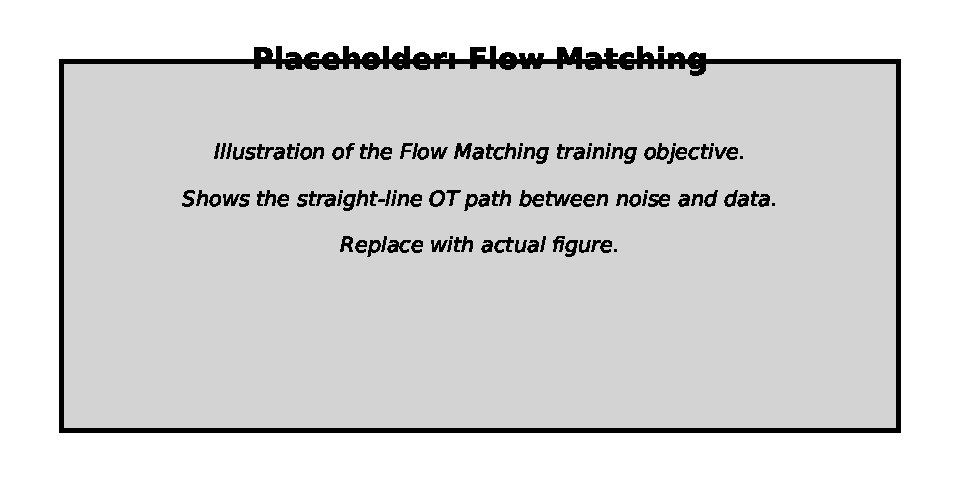
\includegraphics[width=0.8\linewidth]{Figures/figure_flow_matching.pdf}
  \caption{Placeholder: Illustration of the Flow Matching training objective. Replace with a figure showing the straight-line OT path between noise and data.}
  \label{fig:placeholder-flow-matching}
\end{figure}
